\documentclass[UTF8]{article}
\usepackage{ctex}
\usepackage{ulem}
\usepackage{dsfont}
\usepackage{amssymb}
\usepackage{amsmath}
\usepackage{graphicx}
\newtheorem{thm}{定义}[section]
\newtheorem{notation}[thm]{记号}
\newtheorem{lemma}[thm]{引理}

\makeatletter
\newcommand{\rmnum}[1]{\romannumeral #1}
\newcommand{\Rmnum}[1]{\expandafter\@slowromancap\romannumeral #1@}
\makeatother
\newcommand{\dperp}{\perp\!\!\!\perp}

\title{14 $\lambda{\rm D}$中的数字与算术\\Numbers and arithmetic in $\lambda{\rm D}$\\[2ex]\begin{large}读书笔记\end{large}}
\author{许博}
\date{}

\begin{document}
\maketitle
	\section{用于自然数的皮亚诺公理}
	\noindent
	皮亚诺假设存在一个集合$\mathbb{N}$,一个特定的成员0,以及一个由$\mathbb{N}$到$\mathbb{N}$的后继函数$s$。所以在$\mathbb{N}$中,我们有成员0,$s(0)$,$s(s(0))$等,表示0,1,2等。
	
		之后,皮亚诺通过添加公理,使得这些形式化的数字行为符合预期。为了保证函数$s$一定产生新的数字,皮亚诺添加了两条公理:
		
		$ax{-}nat_1:\ \forall_{x\in\mathbb{N}}(s(x)\not=0)$
		
		$ax{-}nat_2:\ \forall_{x,y\in\mathbb{N}}(s(x)=s(y)\Rightarrow x=y)$
		
		公理$ax{-}nat_2$表示$s$是一个单射的函数,而$ax{-}nat_1$隐含了$s$不是满射的。这两条公理决定了不同层数$s$的自然数不相同。
		
		除此之外,皮亚诺还添加了另一条公理,以通过数学归纳法确定所有自然数的性质:
		
		$ax{-}nat_3:\ (P0\land\forall x:\mathbb{N}.(Px\Rightarrow P(sx)))\Rightarrow\forall x:\mathbb{N}.Px$
		
		\begin{lemma} 对于所有$n\in\mathbb{N}:n=0\lor\exists_{m\in\mathbb{N}}(n=s(m))$
		\end{lemma}
	
	\section{以公理方式引入整数}
	\noindent
	整数的公理化假设存在一个$\mathbb{Z}$,一个特定的成员0,以及一个由$\mathbb{Z}$到$\mathbb{Z}$的后继函数$s$。包含如下公理:\\
	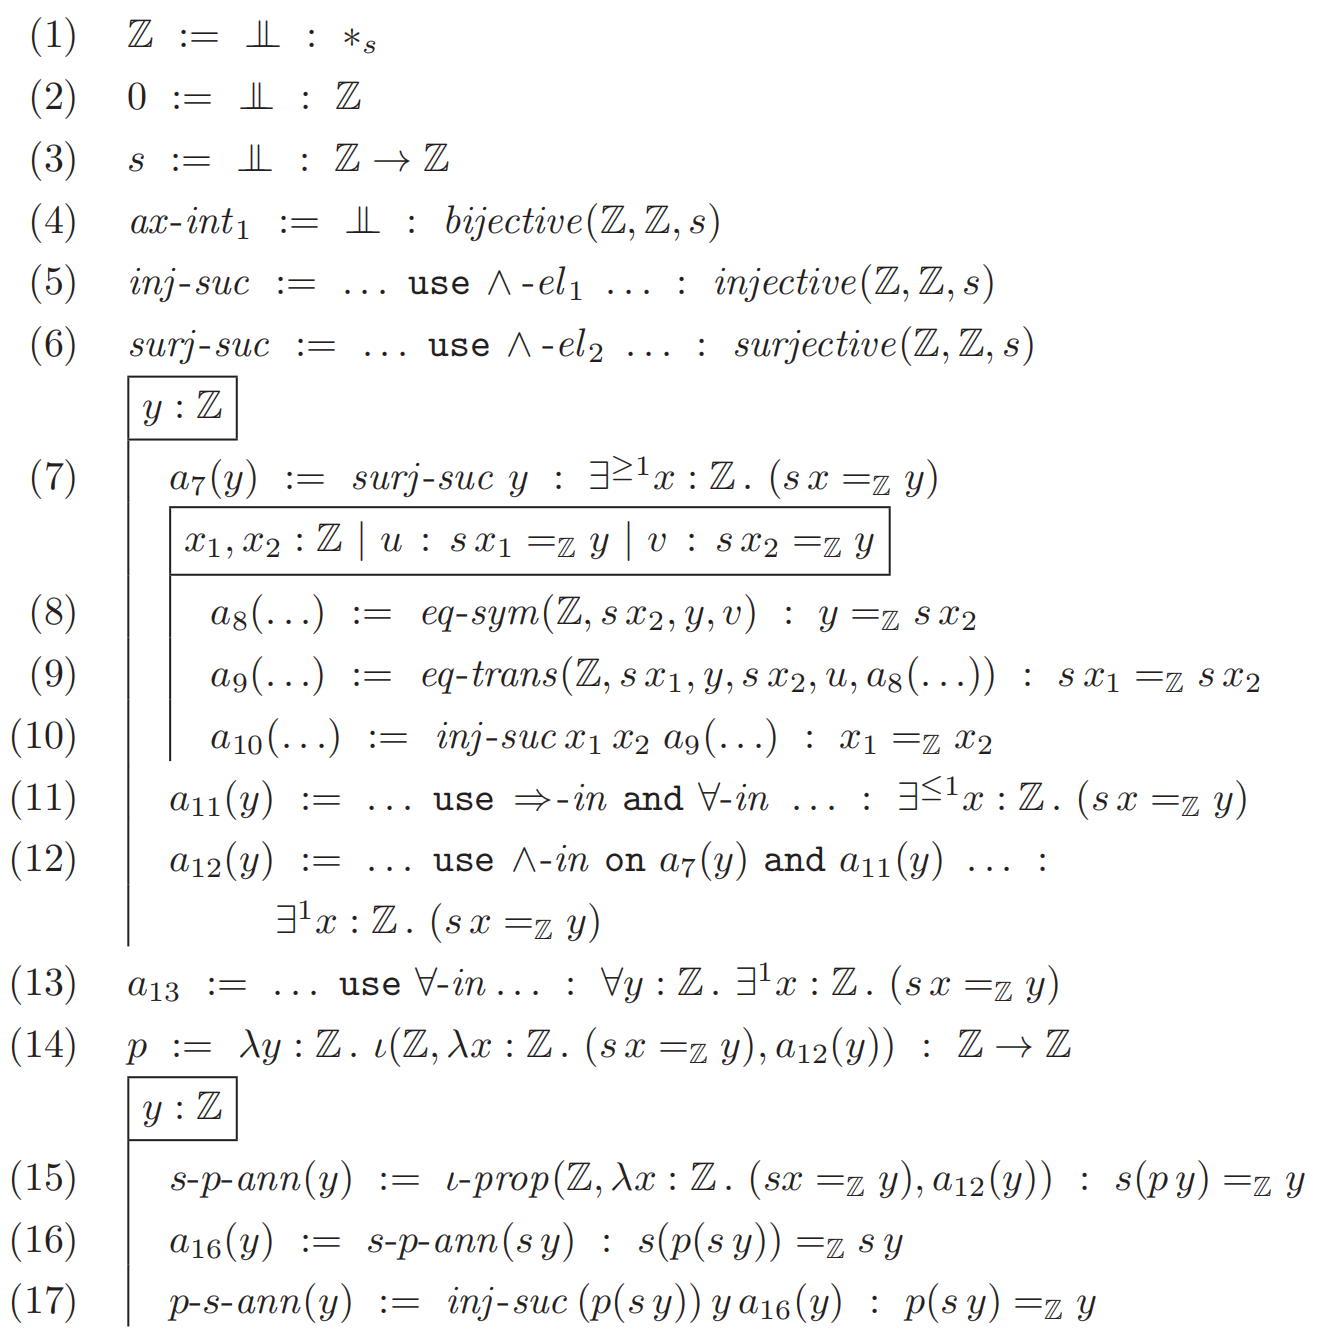
\includegraphics[width=0.93\linewidth]{"../imgs/14-1.png"}
		
		公理$ax{-}int_1$表示$s$是一个双射函数:单射以及满射。由满射性可得,对于所有$y\in\mathbb{Z}$,存在一个$x\in\mathbb{Z}$,使得$s(x)=y$。由单射性可得,$y$确定时,满足$s(x)=y$的$x$是唯一的。
		
		行(14)中定义的$p$,$p(y)$表示$y$的前驱,也即$s(x)=y$中的$x$,可以发现,$p$是$s$的逆函数。
		
		除了上图中出现的公理$ax{-}int_1$,还有公理$ax{-}int_2$,也即用于整数的归纳法,与自然数的版本相比较,在增加了前驱方向的归纳:\\
		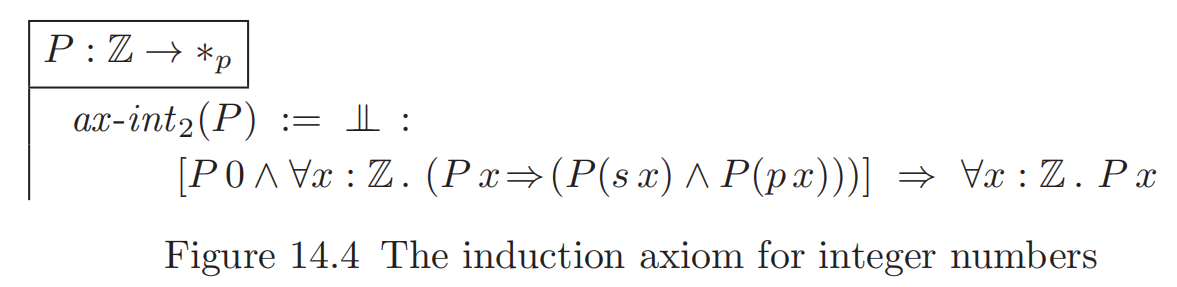
\includegraphics[width=0.93\linewidth]{"../imgs/14-2.png"}
		
		此时我们可以将从0“向上”的整数,也即自然数,作为$\mathbb{Z}$的一个子集$\mathbb{N}$:\\
		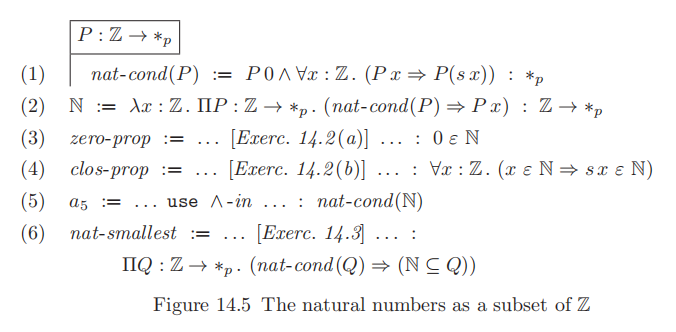
\includegraphics[width=0.93\linewidth]{"../imgs/14-3.png"}
		
		其中$nat{-}cond(P)$表示$P$满足自然数的归纳法的谓词,也即覆盖了所有的自然数,可以看到,如果一个整数$x$对于任意满足$nat{-}cond$的谓词$P$,都有$Px$成立,则$x$是一个自然数。而满足$nat{-}cond$的谓词并不一定只作用于自然数,所以$nat{-}smallest$表示了$\mathbb{N}$是这些子集中的最小子集。
		
		但目前仍存在一个问题,整数集合$\mathbb{Z}$不能保证其的左右是无限的,比如对于集合$\{a,b,c,d\}$,令$a=0$,有$s(a)=b,s(b)=c,s(c)=d,s(d)=a$,$s$同样是双射的,并且适用于归纳法。解决方式是添加一个公理,以确保0的前驱不是自然数:
		
		$ax{-}int_3:=\dperp:\neg(p0\ \varepsilon\ \mathbb{N})$
		
		至此我们拥有了整数,自然数,以及负数。
		
	\section{`新'$\mathbb{N}$的基本性质}
	\noindent
	在`新'的$\mathbb{N}$中,之前的皮亚诺公理依然成立。对于自然数的数学归纳法,需要重新表述为:$(P0\land\forall x:\mathbb{Z}.(x\ \varepsilon\ \mathbb{N}\Rightarrow(Px\Rightarrow P(sx))))\Rightarrow\forall x:\mathbb{Z}.(x\ \varepsilon\ \mathbb{N}\Rightarrow Px)$。
		
		\begin{lemma} $\forall x:\mathbb{Z}.(x\ \varepsilon\ \mathbb{N}\Rightarrow(x=_{\mathbb{Z}}0\lor px\ \varepsilon\ \mathbb{N}))$
		\end{lemma}
	
		\noindent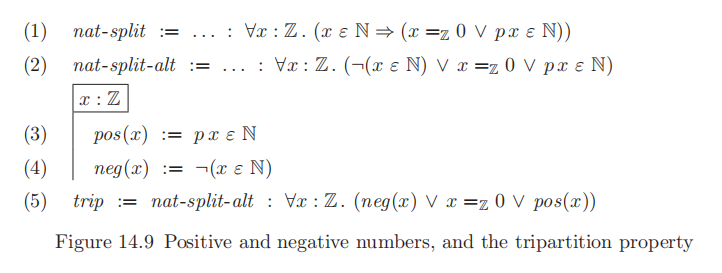
\includegraphics[width=0.93\linewidth]{"../imgs/14-4.png"}\\
		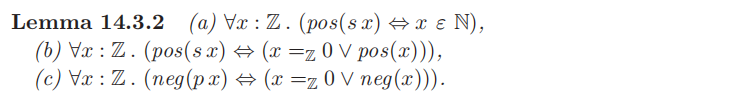
\includegraphics[width=0.93\linewidth]{"../imgs/14-5.png"}\\
		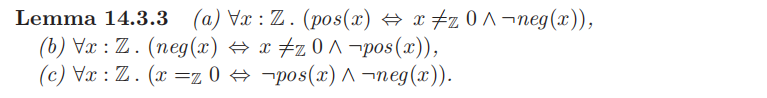
\includegraphics[width=0.93\linewidth]{"../imgs/14-6.png"}
	
	\section{整数加法}
	\noindent
	为了计算形式化的数字,形式化算术运算。首先是加法,通过如下形式的递归定义:
	
		(\rmnum{1}) $m + 0 = m$,
		
		(\rmnum{2}) $m + s(n) = s(m + n)$。
		
		可以发现$m$没有变动,递归基于第二个操作数,因此可以重新表述为:
		
		(\rmnum{1}) $+_m(0)=m$,
		
		(\rmnum{2}) $+_m(s(n))=s(+_m(n))$。
		
		而对于操作数是负数的情况,可以由(ii)推导得到,因此,对于整数而言,这两个定义足够。
		
		用于整数的良构递归定义:\\
		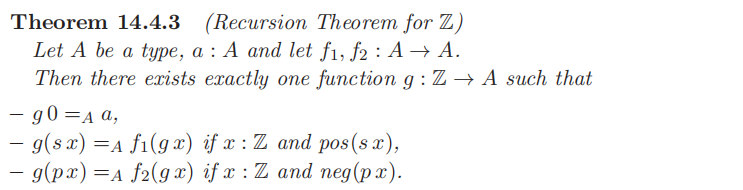
\includegraphics[width=0.93\linewidth]{"../imgs/14-7.png"}
		
		对于一个能够终止的作用于整数集合的递归定义,存在一个唯一的函数$g$满足。形式化为:\\
		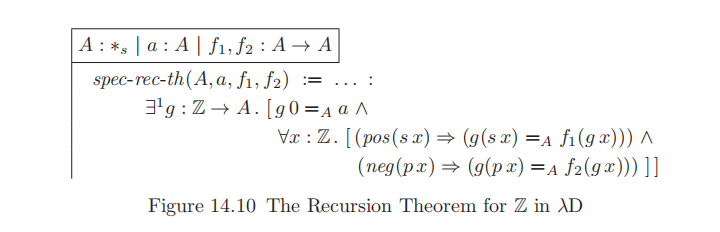
\includegraphics[width=0.93\linewidth]{"../imgs/14-8.png"}
		
		而如果给定的函数$f$是一个双射函数,则可以定义良构递归为:\\
		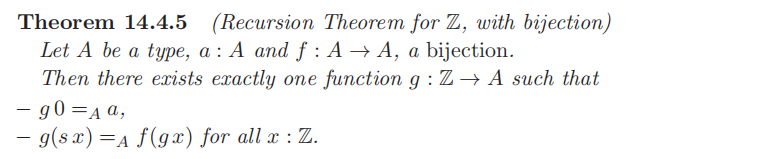
\includegraphics[width=0.93\linewidth]{"../imgs/14-9.png"}
		
		在$\lambda{\rm D}$中形式化$+_m$以及$+$:\\
		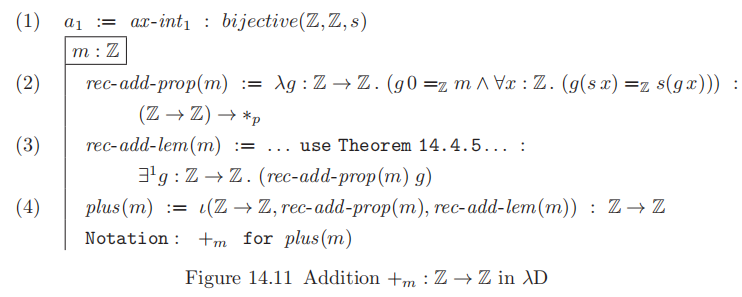
\includegraphics[width=0.93\linewidth]{"../imgs/14-10.png"}\\
		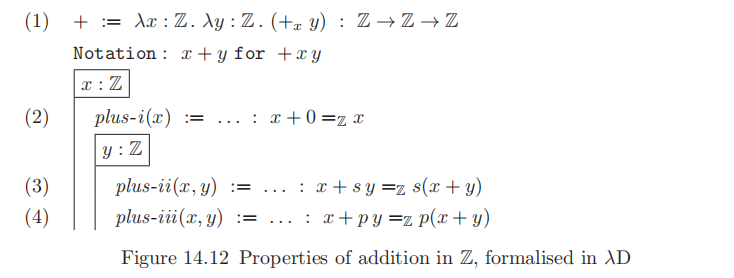
\includegraphics[width=0.93\linewidth]{"../imgs/14-11.png"}
	
	\section{$\lambda{\rm D}$中基础计算的一个例子}
	\noindent
	证明$1+2=3$:\\
	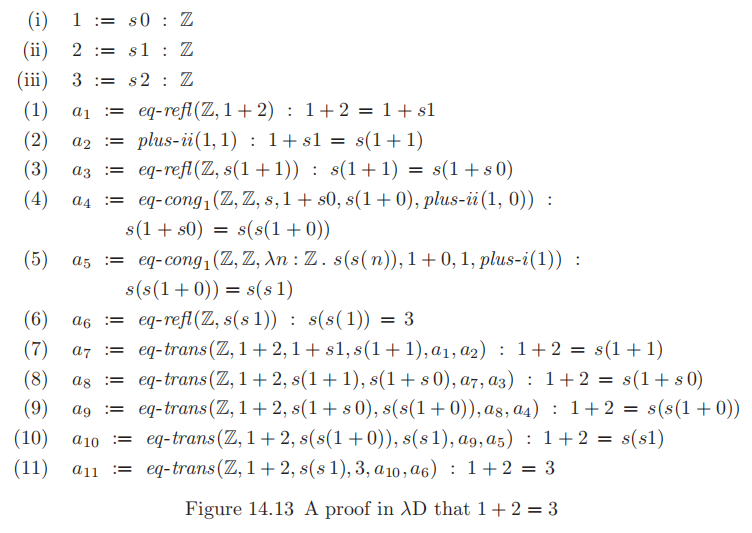
\includegraphics[width=0.93\linewidth]{"../imgs/14-12.png"}
	
	\section{用于加法的算术公理}
	\noindent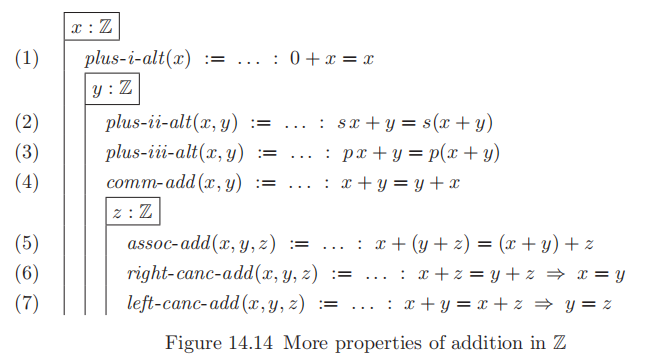
\includegraphics[width=0.93\linewidth]{"../imgs/14-13.png"}
	
	\section{用于自然数和负数的加法下的闭包}
	\noindent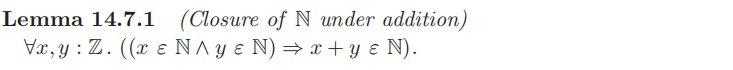
\includegraphics[width=0.93\linewidth]{"../imgs/14-14.png"}\\
	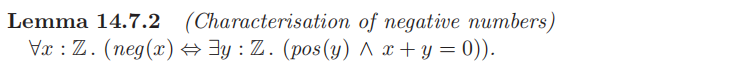
\includegraphics[width=0.93\linewidth]{"../imgs/14-15.png"}\\
	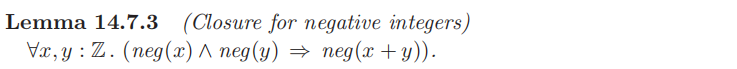
\includegraphics[width=0.93\linewidth]{"../imgs/14-16.png"}
	
	\section{整数减法}
	\noindent
	定义减法:$x-y:=\iota_{z:\mathbb{Z}}(z+y=x)$。性质不再赘述。
	
	\section{整数的相反数}
	\noindent
	定义相反数:$-x:=0-x$。
	
	\section{整数上的非相等关系}
	\noindent
	定义$\le_{\mathbb{Z}}:=\lambda x:\mathbb{Z}.\lambda y:\mathbb{Z}.(y-x\ \varepsilon\ \mathbb{N}):\mathbb{Z}\rightarrow\mathbb{Z}\rightarrow*_p$。\\定义$<_{\mathbb{Z}}:=\lambda x:\mathbb{Z}.\lambda y:\mathbb{Z}.(x\le_{\mathbb{Z}}y\land x\not=y):\mathbb{Z}\rightarrow\mathbb{Z}\rightarrow*_p$。
	
	\section{整数乘法}
	\noindent
	定义乘法为:
	
		(\rmnum{1}) $m·0=0$,
		
		(\rmnum{2}) $m·s(n)=(m·n)+m$。
		
	\section{可除性}
	\noindent
	定义可除性为:$m$可以整除$n$,如果存在$q:\mathbb{Z}$使得$m·q=n$。
	
		需要注意的是,可除性在自然数上是一个偏序关系。
\end{document}
